\documentclass[a4paper,11pt]{article}
\usepackage{exptech}
\usepackage{textcomp}
\usepackage{graphicx}
\usepackage{array}
\usepackage[babel=true]{csquotes}
\usepackage{url}
\usepackage{hyperref}
\usepackage{wrapfig}
\usepackage[export]{adjustbox}
\usepackage{titletoc}

\titlecontents{subsection}[3.8em]{}{}{}{}[\addvspace{-0.5pt}]
\hypersetup{
  pdftitle={Avalon - Rapport de planification}, % title
  pdfnewwindow=true, % links in new window
  colorlinks=true, % false: boxed links; true: colored links
  linkcolor=black, % color of internal links (change box color with linkbordercolor)
  citecolor=cyan, % color of links to bibliography
  filecolor=cyan, % color of file links
  urlcolor=cyan % color of external links
}

\title{
  \textbf{Avalon}\\
  Rapport de planification
}
\markright{Avalon - Rapport de planification }
\author{
\begin{minipage}{0.4\textwidth}
	\begin{flushleft} \large
		\emph{Auteurs :}\\
		Alexandre \textsc{Audinot}\\
		Julien \textsc{Bouvet}\\
		Cyrille \textsc{Delabre}\\
		Thierry \textsc{Gaugry}\\
		Nicolas \textsc{Hurman}\\
		Léo \textsc{Jacoboni}\\
		Alexandre \textsc{Leonardi}\\
	\end{flushleft}
\end{minipage}
\begin{minipage}{0.4\textwidth}
	\begin{flushright} \large
		\emph{Encadrants :} \\
		Valérie \textsc{Gouranton}\\
		Ronan \textsc{Gaugne}\\
		Bruno \textsc{Arnaldi}\\
		Willy \textsc{Allègre}\\
		Jean-Paul  \textsc{Departe}\\
	\end{flushright}
\end{minipage}
}

\date{17 Décembre 2014}

\begin{document}
\maketitle
\thispagestyle{empty}


%\vfill
%[width=\textwidth]
\begin{figure}[h!]
   \begin{minipage}{0.3\linewidth}
      
\includegraphics[scale=0.9]{3-Planification/img/logo_insa.jpeg}
   \end{minipage} 
   \begin{minipage}{0.2\linewidth}
      \centering
      
\includegraphics[scale=0.5,left]{3-Planification/img/logo_irisa.jpg}
   \end{minipage}\hfill
   \begin{minipage}{0.2\linewidth}
      
\includegraphics[scale=0.9]{3-Planification/img/logo_kerpape.png}
   \end{minipage}
\end{figure}

\pagebreak

\tableofcontents
\pagebreak

\section{Introduction}
Dans le cadre de notre projet 4INFO, nous allons réaliser une application pour le Centre de de rééducation fonctionnelle de Kerpape. Il s'agit de modéliser des appartements tremplins qui sont spécialement équipés pour que les personnes handicapées puissent y vivre en toute autonomie. Ils servent à les préparer à reprendre une vie normale dans des appartements lourdement équipés en domotique. Le problème est que le centre ne dispose que de deux appartements tremplins, ce qui n'est pas suffisant pour le nombre de leurs patients.\newline

De plus, le nombre important des équipements automatisés pose des problèmes d'apprentissage, particulièrement pour les personnes ayant des troubles cognitifs. De ce fait, l'objectif de notre application est de fournir aux patients, ainsi qu'aux thérapeutes qui les accompagnent, un outil informatique qui leur permettra de se familiariser avec les équipements des appartements avant le test \textit{in situ}. \newline

Notre application implémentera notamment les fonctionnalités suivantes :
\begin{itemize}\renewcommand{\labelitemi}{$\bullet$}
	\item 3 modes d'apprentissage, chacun avec un niveau de réalisme différent, qui permettent d'aller d'une prise en main basique à une totale liberté
	\item 3 scénarios prédéfinis mettant en scène l'utilisation du combiné téléphone/interphone
 	\item Le support de différents périphériques d'utilisation (clavier/souris, Oculus Rift, salle de réalité virtuelle Immersia)
\end{itemize}
\vspace{0.5cm}
\hspace{0.5cm}L'ensemble de nos spécifications (détaillées dans le rapport précédent) nous ont permis d'aiguiller la planification de ce projet présentée dans ce rapport.
\pagebreak
\section{Contexte}

\subsection{Qu'est-ce que la réalité virtuelle ?}La notion de réalité virtuelle, contrairement à ce que l'on pourrait penser, n'est pas récente et date du début des années 80 quand Jaron Lanier, un informaticien américain pionnier du domaine, l'a popularisée. Cette notion n'a pourtant pas, à l'origine, l'exact sens qu'on lui prête habituellement aujourd'hui : une réalité virtuelle sous-entendrait qu'il s'agit d'une copie exacte de la réalité, ce qui n'est jamais le cas, faute de moyens techniques, et n'est pas toujours recherché. Le terme venant  de l'anglais, \emph{virtual} peut se traduire par \emph{virtuelle} mais aussi par \emph{quasi} ou \emph{pratiquement}, or cette notion de \emph{quasi-réalité} correspondrait mieux à ce qu'est effectivement la réalité virtuelle. \\

En effet, de manière plus formelle, on peut définir la réalité virtuelle comme suit :

\begin{quote}\og \emph{La réalité virtuelle est un domaine scientifique et technique exploitant l'informatique et les interfaces comportementales en vue de simuler dans un monde virtuel le comportement d'entités 3D, qui sont en interaction en temps réel entre elles et avec un ou des utilisateurs en immersion pseudo-naturelles par l'intermédiaire de canaux sensori-moteurs.} \fg{}\end{quote}\cite{traiteRV1}

%Il faudra penser à citer la source : Le traité de la RV
Cela signifie que pour que l'on puisse parler de réalité virtuelle il faut que plusieurs conditions soient réunies :
\\
\begin{itemize}\renewcommand{\labelitemi}{$\bullet$}
\item \textbf{La présence d'interfaces comportementales et sensorielles. }
Les interfaces comportementales désignent les interfaces entre l'utilisateur et le monde virtuel. Il existe dans un premier temps des interfaces motrices, qui permettent de reconnaître les différentes actions que l'utilisateur peut entreprendre (mouvements, voix, etc). Ainsi le système informatique gérant le monde virtuel peut alors les prendre en compte. Les interfaces sensorielles font ensuite la liaison opposée et informent l'utilisateur de l'état du monde virtuel et des modifications éventuelles des actions entreprises précédemment (images, sons, etc). La réciprocité du besoin d'une interface motrice et sensorielle, qui sont nécessaires pour l'immersion du sujet et permettent de gérer l'interaction avec le monde virtuel, est illustrée par la \textsc{figure 1}.
\item \textbf{L'immersion du sujet.}
L'immersion caractérise le fait que les interfaces entre l'utilisateur et le monde virtuel doivent se faire oublier, et ce, en ressemblant le plus possible aux méthodes d'interaction que nous avons avec le monde réel. Elle ne peut pas être parfaite, car il y a toujours du matériel à utiliser qui n'est pas nécessaire pour interagir avec le monde réel (lunettes 3D, WiiMote, etc) mais doit être la plus totale possible.\\

\end{itemize}
\begin{figure}
  \caption{Interactions entre monde réel et virtuel \cite{traiteRV1}}
  %\centering
  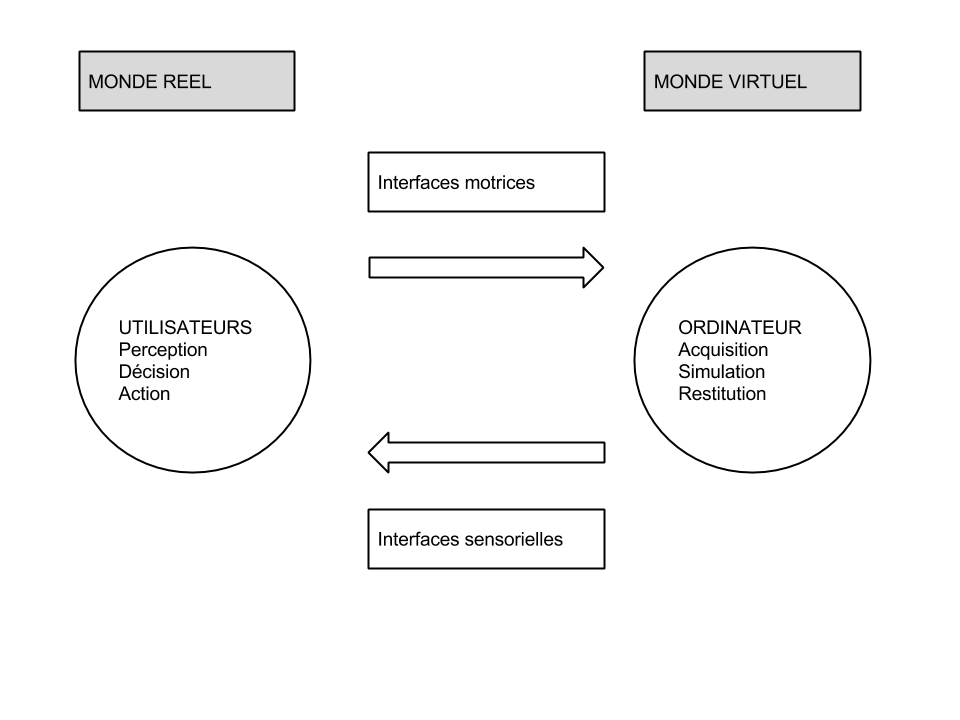
\includegraphics[scale=0.4,bb=0 0 720 720]{1-PreEtude/img/graphe_interfaces.png}
\end{figure}

La notion de réalité virtuelle implique donc également celles d'immersion et d'interaction, elles sont en fait constitutives de ce qu'est la réalité virtuelle. L'utilisateur doit pouvoir faire des actions motrices sur son environnement, il doit pouvoir agir dessus que ce soit par les mouvements, la parole, les gestes... Il n'y a pas de règles définies tant qu'il s'agit d'une activité motrice.
Une activité sensorielle, par ailleurs, signifie que l'utilisateur percevra un impact de ses actions sur le monde virtuel. Encore une fois il n'y a pas de liste de réponses sensorielles acceptables, ce peut être un son ou encore une modification de l'affichage.


\subsection{La Réalité Virtuelle et l'aide à la personne}

\subsubsection{L'aide à la personne}

Notre projet va traiter d'une application bien particulière de la réalité virtuelle (RV) : la santé. La RV est déjà utilisée dans le cadre de la santé et des soins. Les psychologues s'en servent par exemple pour traiter les cas de phobie, car une application de réalité virtuelle leur permet de plonger leurs patients dans la situation qui est l'objet de leur peur facilement, mais aussi de la garder sous contrôle et de la reproduire rapidement et à peu de frais. Le même avantage s'applique au traitement de l'autisme chez les enfants, car la RV permet de simuler des situations qui s'avéreraient dangereuses et qu'ils ne savent pas gérer, comme traverser une route seuls.\cite{traiteRV4}\\

Notre projet a été proposé par le centre de rééducation et de réadaptation fonctionnelle de Kerpape, et se focalisera donc sur le domaine d'expertise du centre, à savoir l'aide aux personnes handicapées. Le principe de l'aide à la personne est d'assister des personnes âgées ou handicapées dans les gestes de tous les jours, pour leur permettre de conserver leur autonomie.

\subsubsection{Le centre de Kerpape}

Nous avons eu l'occasion de visiter le centre de Kerpape au cours de notre projet. Kerpape accueille 400 patients chaque jour, et a pour objectif de leur permettre d'acquérir l'autonomie nécessaire à une réinsertion sociale et professionnelle. \\
Du fait de la grande diversité des handicaps que présentent les patients du centre, la modification du matériel existant est un pan important du travail de Willy Allègre et Jean-Paul Departe, les ingénieurs commanditaires de notre projet, et cela rend la RV particulièrement intéressante, un logiciel étant plus facilement reconfigurable que du matériel.\cite{kerpape}\\


C'est le second projet de RV auquel participe le centre de Kerpape. Le premier était le projet AGATHE, débuté en 2009, dont le but est d'aider les personnes atteintes de troubles cognitifs (par exemple dus à la maladie d'Alzheimer, à des AVC, ...) à être autonomes dans la vie de tous les jours. Le projet consiste en la réalisation d'un \og voisinage virtuel \fg{} dans lequel le patient peut se déplacer, et où se trouvent plusieurs points d'intérêts avec lesquels il peut interagir, tel qu'un bureau de poste, un supermarché, etc. Le patient a donc accès à différentes actions en accord avec le lieu dans lequel il se trouve, et le thérapeute peut évaluer ses performances en fonction de plusieurs critères comme le temps passé par le patient dans une zone donnée.\cite{agathe}

\subsubsection{Le projet Avalon}

Le projet qui nous a été confié, le projet Avalon, est le premier projet de collaboration entre Kerpape et l'INSA. Il a aussi pour but d'aider les personnes handicapées à recouvrer leur autonomie, mais il se focalise sur un aspect différent de la vie de tous les jours : l'utilisation de la domotique dans l'habitat des patients. Durant leur phase de rééducation au centre de Kerpape, les patients sont amenés à vivre quelques temps dans un appartement \enquote{tremplin} appartenant au centre. Ces appartements sont lourdement équipés en domotique pour que des personnes handicapées puissent y être autonomes, les différentes portes, fenêtres et volets sont contrôlables à distance par différents interrupteurs, un plan de travail dans la cuisine est réglable en hauteur, un mobile accroché à des rails au plafond aide les déplacements, etc.
Les appartements tremplins servent à présenter aux patients les différents équipement disponibles pour leur propre appartement une fois qu'ils quitteront le centre, mais aussi à les entraîner à l'usage de ces équipements, qui peut s'avérer complexe, particulièrement pour les personnes souffrant de handicaps mentaux. \\

Le centre de Kerpape a donc initié le projet Avalon pour permettre aux patients de se préparer à l'utilisation des appartements même si ceux-ci sont occupés, et pour que les thérapeutes encadrant les patients puissent profiter de différents modes d'utilisation leur permettant de se focaliser sur les interactions les plus problématiques, comme détaillé dans le cahier des charges.

\pagebreak
\section{Méthodes d'organisation \& planification}
\pagebreak
\section{Planification Microsoft Project}

Microsoft Project est un outil puissant, que nous apprenons tout juste à appréhender. Il nous offre un grand nombre de possibilités ainsi qu'une aide qui s'avérera utile dans le pilotage de notre projet. Nous avons retenu les informations les plus importantes qu'il synthétise.

\subsection{Chronologie du projet}
Cette vue est la plus synthétique que nous ayons réalisée, elle donne une vue d’ensemble du projet ne comprenant que les plus grandes étapes. \newline
\emph{Mettre ici chronologie générale}\newline

Une autre vue importante tout en restant synthétique est la liste des jalons qui structurent le développement de notre application.\newline
\emph{Mettre les jalons à respecter}

\subsection{Affectation des ressources par tâche}
Nous avons subdivisé notre projet en un ensemble de sous-tâches avec le plus de précision possible, en tentant de faire une estimation de la durée que chacune d'entre elle demanderait.\newline

Le diagramme suivant résume le temps requis par chaque tâche, en prenant en compte notre nombre ainsi que le travail que nous pourrons fournir selon les semaines (semaine d'examens, semaine réservée au projet, etc).\newline
\emph{Mettre la répartition du temps de travail par partie}

\subsection{Diagramme de Gantt}
Le diagramme de Gantt permet d'avoir une vue plus détaillée des différentes tâches du projet, ordonnancées en fonction de leur durée et de leur priorité. \newline
\emph{Mettre le diagramme de Gantt}
\pagebreak
\section{Évaluation des risques}

Il s'agit de la dernière étape de la planification du projet Avalon : l’évaluation des risques qui pourraient survenir, ainsi que la solution à adopter le cas échéant. Nous les avons classés en 3 catégories, les risques humains, les risques techniques, et ceux liés à une mauvaise gestion du projet. 

\subsection{Risques humains}
Des erreurs ou des actions malintentionnées que quelqu'un pourrait commettre. \newline

\textbf{Vol de matériel}
\newline
C'est sans doute du risque le plus grave mais aussi le moins probable. Un vol de matériel, par exemple le vol de notre Oculus Rift, serait extrêmement préjudiciable : le matériel est cher et compliqué à remplacer, mais aussi nécessaire pour la réalisation du projet et la conduite de tests. Dans ce cas-là, nous demanderions au département Informatique ou à l'IRISA de nous prêter le matériel manquant.\newline
Néanmoins, ce cas de figure a peu de chances de se réaliser car la salle $\mu$RV est verrouillée dès que personne ne l'occupe.\newline

\textbf{Perte de données}
\newline
Évantualité déjà plus probable, la perte de données est censée être peut s'avérer elle aussi assez handicapante, en fonction de la quantité de données ainsi disparues. Cependant, l'utilisation d'un gestionnaire de version est censée prévenir ce type de déboires.\newline
Il peut toujours arriver que cela ne suffise pas, et dans ce cas-là il n'y a guère de solutions pour récupérer ce qui a été perdu. Cependant, le \emph{commit} régulier des modifications fait que ce ne sont que de petites portions de codes qui sont sujettes à ce risque.\newline

\subsection{Risques techniques}
Ce sont les risques ne dépendant des membres du groupe ou d'une autre personne. Ils sont liés aux machines ou logiciels utilisés.\newline

\textbf{Dépôt Git indisponible}
\newline
Nous utilisons Git comme gestionnaire de versions pour le travail collaboratif. Cependant, chaque membre possédant une copie du projet au complet sur son disque dur, nous pourrions changer de gestionnaire de versions dans le cas d'un problème persistant ou partager le code directement \emph{via} clé USB dans le cas d'un problème ponctuel.\newline

\textbf{Pannes}
\newline
Les pannes de matériel peuvent avoir une incidence variable. Une panne d'un PC sera sans impact car nous en avons suffisamment à disposition pour que cela ne nous retarde pas ; la panne d'un dispositif unique comme l'Oculus Rift s'avérera en revanche plus problématique.\newline
Dans ce cas comme dans le cas du vol, la solution consiste à demander au département informatique ou à l'IRISA de nous prêter du matériel pour remplacer celui qui est en panne.\newline

\subsection{Risques quant à la gestion du projet}
Une mauvaise gestion du projet pourrait conduire à des problèmes épineux. Il peut être compliqué de découvrir le problème avant qu'il ait pris une certaine ampleur. \newline

\textbf{Clients insatisfaits}
\newline
Dans le cas où l'application finale ne conviendrait pas au centre de Kerpape, il pourrait être trop tard pour effectuer les changements qui seraient attendu. C'est la raison pour laquelle nous avons décidé d'adopter une méthode de développement agile, en présentant régulièrement nos avancées à Jean-Paul Departe et Willy Allègre. Ainsi, si une partie du projet ne leur convient pas, nous sommes sûrs de le détecter suffisamment tôt. \newline

\textbf{Sous-estimation de la complexité d'une tâche}
\newline
Un risque inhérent à notre manque d'expérience avec des projets de cette ampleur : il est parfois difficile d'estimer la durée que prendra une tâche et les difficultés qu'elle présentera. Notre planning tient compte de cette possibilité et les estimations de temps ont été faites en conséquence.\newline

\pagebreak
\section{Conclusion}

Nous avons donc choisi une méthode fortement inspirée du cycle de production en V mais en la mêlant à des méthodes agiles pour pouvoir présenter le projet à nos clients régulièrement. Ainsi si chaque jalon du projet, représenté par un livrable à rendre, correspond à une étape de notre cycle en V, nous prévoyons en parallèle d'avancer le développement de l'application, en en présentant les itérations successives à Jean-Paul Departe et Willy Allègre. \newline

Ainsi, nos commanditaires peuvent valider notre avancée en quasi-temps réel. De plus, d'après l'audit réalisé sur Microsoft Project, nous disposons d'une planification correcte. Les différents livrables seront réalisés dans les temps et les estimations que nous avons faites tiennent compte des contre-temps que nous sommes susceptibles de rencontrer et devraient suffire à absorber les retards.

\end{document}
